% This file was created with tikzplotlib v0.10.1.
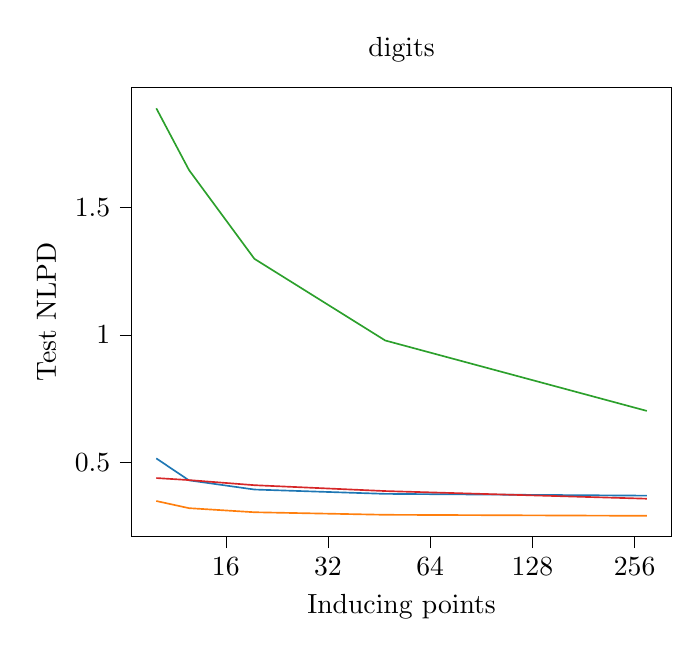
\begin{tikzpicture}

\definecolor{crimson2143940}{RGB}{214,39,40}
\definecolor{darkgray176}{RGB}{176,176,176}
\definecolor{darkorange25512714}{RGB}{255,127,14}
\definecolor{forestgreen4416044}{RGB}{44,160,44}
\definecolor{steelblue31119180}{RGB}{31,119,180}

\begin{axis}[
tick align=outside,
tick pos=left,
title={digits},
x grid style={darkgray176},
xlabel={Inducing points},
xmin=4, xmax=268,
xtick style={color=black},
xtick={0,50,100,150,200,250,300},
xticklabels={0,16,32,64,128,256,},
y grid style={darkgray176},
ylabel={Test NLPD},
ymin=0.21115, ymax=1.96785,
ytick style={color=black}
]
\addplot [semithick, steelblue31119180]
table {%
16 0.516
32 0.43
64 0.394
128 0.377
256 0.37
};
\addplot [semithick, darkorange25512714]
table {%
16 0.349
32 0.321
64 0.305
128 0.295
256 0.291
};
\addplot [semithick, forestgreen4416044]
table {%
16 1.888
32 1.646
64 1.298
128 0.978
256 0.702
};
\addplot [semithick, crimson2143940]
table {%
16 0.439
32 0.431
64 0.411
128 0.388
256 0.358
};
\end{axis}

\end{tikzpicture}
